\documentclass[a4paper, 8pt]{article}
\usepackage[T1]{fontenc}
\usepackage[utf8]{inputenc}
\usepackage{lmodern}
\usepackage[spanish]{babel}
\usepackage{graphicx}

	\addtolength{\oddsidemargin}{-.875in}
	\addtolength{\evensidemargin}{-.875in}
	\addtolength{\textwidth}{1.75in}

	\addtolength{\topmargin}{-.875in}
	\addtolength{\textheight}{1.75in}


\title{Trabajo práctico de S.O I \\ Sistema de archivos distribuido}

\begin{document}

\maketitle

\section{Implementación en C con POSIX Threads}

\subsection{Comunicación entre \textit{workers}}

Creamos 5 hilos en el arranque del sistema, estos se encargan de realizar los pedidos del cliente, los llamamos \textit{workers}.
Asignamos a cada \textit{worker} una cola de mensajes propia (utilizamos Posix Messages Queues para comunicar los a los \textit{workers} entre si).

Cuando un cliente se conecta, lanzamos un hilo, el cual atiende los pedidos del cliente, \textit{proceso socket}.
Este hilo también posee una cola de mensajes propia.
Como muestra la Figura 1, cada \textit{worker} se comunica con los \textit{workers} adyacentes y un proceso socket (si existe).


Ante una llamada al sistema, el proceso socket, enviará la consulta a la cola de mensajes del \textit{worker} X, elegido pseudoaleatoriamente
entre los \textit{workers} que están desocupados.
Luego, el \textit{worker} X responderá al pedido, enviando el resultado a la cola de mensajes del proceso socket,
previo a emitir un mensaje por el anillo, para consultar a los demás workers, si es necesario.


 \begin{figure}[htbp]
   \centering
     \includegraphics[scale=0.75]{dia22.png}
     \caption{Comunicación en anillo entre \textit{workers}}
   \label{Figura 1}
 \end{figure}

\subsection{Estructuras de datos}
\begin{enumerate}
\item Representamos a los mensajes enviados por procesos sockets o \textit{workers} mediante la siguiente estructura:
\begin{verbatim}
typedef struct msj_{
  char tipo;
  char contador;
  char dato;
  int otrodato;
  char *nombre;
  char *texto;
} Msj;
\end{verbatim}

\newpage
Interpretamos a sus miembros de la siguiente manera:

\begin{itemize}
  \item \texttt{tipo}: indica si se trata de un mensaje entre los \textit{workers}, o entre el proceso socket y un \textit{worker}.
  \item \texttt{contador}: varia entre los caracteres \texttt{'0'} y \texttt{'5'}. Lo usamos para identificar al worker que tiene como destino.
  \item \texttt{dato}: por lo general, indica el resultado de un pedido, si fue exitoso o no.
  \item \texttt{otrodato}: contiene el tamaño en bytes del miembro \texttt{texto}. Es útil para los operadores \texttt{REA} y \texttt{WRT}.
  \item \texttt{nombre}: el nombre de uno o varios archivos.
  \item \texttt{texto}: formará parte del contenido de un archivo.
\end{itemize}

\item Representamos a los archivos mediante la siguiente estructura:

\begin{verbatim}
typedef struct archivo_ {
	    char *nombre;
	    char *texto;
	    int estado;
	    int indice;
	    int tam;
	    struct archivo_ *proximo;
} Archivo;
\end{verbatim}

Interpretamos a sus miembros de la siguiente manera:

\begin{itemize}
  \item \texttt{nombre}: el nombre del archivo.
  \item \texttt{texto}: el buffer del archivo.
  \item \texttt{estado}: puede ser 0 o 1, indica si el archivo está cerrado o abierto, respectivamente.
  \item \texttt{indice}: la posición del cursor de lectura.
  \item \texttt{tam}: el tamaño en bytes del archivo.
\end{itemize}

\end{enumerate}

\subsection{Problemas y soluciones}
  \begin{enumerate}
    \item La elección del descriptor de archivos.
    
    Creamos una función con el nombre \texttt{ins\_descriptor}, que retornar el valor de una variable global, antes de ser incrementada.
    Cuando es llamada por el proceso socket, ante el pedido de apertura de un archivo, este hilo, utiliza el valor que obtiene de \texttt{ins\_descriptor} como descriptor de un archivo.
    
    \item Cerrar todos los archivos abiertos por un cliente.
    
    Creamos una lista enlazada global: \texttt{descriptores}, mediante la estructura llamada \texttt{ListaDescriptores}. Contiene los nombres de todos los archivos abiertos, junto a los \textit{workers} a los pertenecen, entre otros datos.
    Creamos operadores que actúan sobre \texttt{ListaDescriptores}.
    En su implementación tuvimos en cuenta el uso de \textit{memory barriers}.
    Con la función \texttt{buscar\_descriptor}, podemos filtrar los nombres de los archivos abiertos por un cliente determinado que desee desconectarse, para luego cerrarlos.
    
    \item La comunicación entre un proceso socket y un FS.
    
    En un principio, el hilo que atendía los pedidos tenia que tomar el mensaje enviado por un \textit{worker} directamente de la cola de mensajes de este \textit{worker};
    no habíamos creado una cola de mensajes para cada proceso socket. 
    Entonces, consulta y respuesta se enviaban a la misma cola de mensajes. Lo cual generaba ciertos inconvenientes. Por ejemplo,
    un \textit{worker} podría leer el mismo mensaje que había enviado, o un proceso socket tendría la chance de
    leer un mensaje emitido solo para circular por el anillo.
    Por lo tanto, decidimos asignarle una cola de mensajes a cada proceso socket, a medida que éstos son lanzados.
    
    \item Pedidos concurrentes de creación de archivos con el mismo nombre.
    
    Cuando un \textit{worker} recibe el pedido de creación de un archivo, debe consultar a los demás. Entonces, cada \textit{worker} revisa su lista de archivos, para
    determinar si el archivo ya existe. Hasta este punto, nuestra comunicación en anillo, permitiría la creación de archivos duplicados.
    Añadimos lo siguiente:
    cuando un \textit{worker} es consultado, además de revisar su lista de archivos, examina si tiene pendiente un pedido de creación de archivo,
    y si el nombre de éste coincide con el nombre del archivo buscado.
    %Si no tenemos en cuenta este punto, nuestro sistema de anillos, permitiría la creación de archivos duplicados. Decimos prevenirlo advirtiendo a los clientes con un error,
    
%     \item Liberar la memoria asignada dinámicamente a un mensaje.
    
%     Dados \texttt{p1 :: Msj*} y \texttt{p2 :: char*}.
    
%     Realizábamos los siguientes pasos para enviar y recibir un mensaje:
    
%     \begin{enumerate}
%       \item Asigamos memoria a \texttt{p1}, e inicializamos.
%       \item Castemos \texttt{p1} tal que \texttt{p1 :: char*}, y lo pasamos como argumento a \texttt{mq\_send}.
%       \item Liberamos la memoria asignada a \texttt{p1}, no asi sus miembros, pues en la cola de mensaje tenemos una copia de lo apuntado por \texttt{p1}.
%       \item Asignamos memoria a \texttt{p2}.
%       \item Pasamos a \texttt{p2} como argumento de \texttt{mq\_receive}, y lo casteamos tal que \texttt{p2 :: Msj*}.
%       \item Trabajamos con \texttt{p2}, y luego liberamos la memoria asignada a \texttt{p2}.
%     \end{enumerate}
    
%     Luego, el proceso se interrumpía abortando.
%     Creemos que en el ultimo paso, liberamos memoria reservada a otro puntero que no es \texttt{p2}. Asi que desistimos de realizar el paso (\textit{f}), y se solucionó.
  \end{enumerate}


\section{Implementación en Erlang}

Realizamos los siguientes puntos adicionales.

\begin{itemize}
  \item Permitimos la apertura de sólo lectura y sólo escritura, dejando múltiples aperturas en modo lectura, y a lo sumo
  una apertura en modo lectura y escritura.
  
  Para ello, modificamos la forma del operador \texttt{OPN} :
  \texttt{OPN MODE ARG1 ARG2}. Ahora, este operador abre el archivo \texttt{ARG2}, en el modo \texttt{ARG1},
  donde \texttt{ARG1} puede ser \texttt{RDONLY} o \texttt{RDWR}.
  
  \item Implementamos el operador \texttt{RM}, de la forma
  \texttt{RM ARG1}. El archivo \texttt{ARG1} será borrado una vez que ya no se mantenga abierto por ningún cliente.
  
  \item Mensajería tolerante a fallas. Si un worker no responde al proceso socket, o el proceso socket no atiende
  al cliente, luego de aprox. 100 ms, el cliente recibirá el siguiente mensaje: \texttt{ERROR 62 ETIME}.
 
\end{itemize}

  \subsection{Comunicación entre workers}
  Reutilizamos parte del código del ejercicio 8, de la práctica de Erlang, en el cual debíamos implementar un Broadcaster.
  Esto nos permite comunicar cada worker con todos los demás, mediante un único proceso (lo llamamos broadcaster).
  
  Cuando uno de los workers quiere consultar a lo otros, envía el pedido al broadcaster. Este se encarga de retransmitir el pedido
  a los 4 workers restantes, y juntar las respuestas en un solo mensaje, que luego transfiere al worker
  que inicio la consulta.
  
 \begin{figure}[htbp]
   \centering
     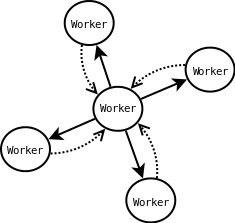
\includegraphics[scale=0.75]{dia2}
     \caption{Sistema de broadcast}
   \label{Figura 2}
 \end{figure}
  
  
\subsection{Estructura de datos}

  Implementamos un archivo con una tupla de la forma:

\vspace{2.5mm}

\{\{ \framebox[3.5\width]{1} , \framebox[3.5\width]{2} \}, \{ \texttt{nombre} , \framebox[3.5\width]{3} \}, \{ \texttt{data} , \framebox[3.5\width]{4} , \framebox[3.5\width]{5} , \framebox[3.5\width]{6} \}\}.

\vspace{2.5mm}

\begin{enumerate}
  \item Atomo, que puede ser \texttt{cerrado}, \texttt{l} o \texttt{lye}. Indica que el archivo no fue abierto por ningún cliente, o el modo de apertura del último cliente,
  con una salvedad:  si es abierto en modo lectura y escritura por un cliente \texttt{C}, este campo no cambia hasta que \texttt{C} lo cierre.
  \item Atomo, que puede ser \texttt{true} o \texttt{false}. Indica si puede borrarse por pedido del operador \texttt{RM}.
  \item Atomo, que tiene el nombre del archivo.
  \item Buffer del archivo, una lista.
  \item Lista de tuplas, con el índice de lectura asociado a un Pid (de un proceso socket).
  \item Tamaño en bytes del buffer dado en el punto 4.
\end{enumerate}

\subsection{Problemas y soluciones}

\begin{enumerate}
%   \item El caracter \texttt{'}$\backslash$\texttt{r} \texttt{'} que añade telnet en el fin de linea.
%   
%   Al principio, no lo tuvimos en cuenta. Por ejemplo, no lograbamos matchear \texttt{"BYE$\backslash \texttt{r}\backslash \texttt{n}$"} con \texttt{"BYE$\backslash \texttt{n}$"}.
%   
  \item Cerrar todos lo archivos abiertos por un cliente.
  
  Para solucionarlo creamos una lista de tuplas de la forma \{\texttt{N},\texttt{M},\texttt{P}\}. Así interpretamos las variables:
  
  \begin{itemize}
    \item \texttt{N}: Atomo que tiene el nombre de un archivo.
    \item \texttt{M}: Atomo que denota el modo de apertura del archivo con nombre \texttt{N}.
    \item \texttt{P}: Pid del \textit{worker} que tiene el archivo \texttt{N}.
  \end{itemize}
  
  Pasamos la lista por argumento a la función \texttt{proc\_socket}, para de mantener los
  nombres de los archivos abiertos, junto a los FS a los que pertenecen.
  Luego, cada archivo que se abre o cierra, añade o elimina respectivamente, un elemento de la lista, con el fin de mantenerla actualizada.
  
  \item Soportar múltiples índices de lectura para un archivo.
  
  Este problema surge a raíz de la implementación de uno de los puntos adicionales. Tenemos que mantener un índice de lectura para cada cliente,
  incluso si todos leen el mismo archivo.
  Entonces, creamos en la tupla que representa un archivo, una lista de tuplas \{\texttt{P},\texttt{I}\} (como vimos en el sección 2.2).
  
  \begin{itemize}
    \item \texttt{P}: es un Pid.
    \item \texttt{I}: un número.
  \end{itemize}
  
  Con esta tupla identificamos el índice \texttt{I} del cliente que tiene como proceso socket aquel con pid \texttt{P}.
  Actualizamos la lista, con la apertura, cierre o lectura del archivo por parte de un cliente, añadiendo, quitando o modificando la tupla correspondiente.
\end{enumerate}

\section{Observaciones}

En ambas implementaciones:

\begin{itemize}

%   \item No se acepta la creación de archivos con nombres que incluyan espacios.
% 
%   \item No son admisibles operaciones con caracteres cuya codificación en UTF-8 requiera más de un byte.
  \item Asumo que cada \textit{worker}, atiende a lo sumo a un solo proceso en un momento dado. Por lo tanto, solo puede haber
  hasta 5 clientes a la vez.

  \item Solo es posible la comunicación cliente-servidor mediante el protocolo telnet.
  
  \item En la operación \texttt{WRT FD ARG0 SIZE ARG1 ARG2}, consideramos a los espacios contiguos en el buffer \texttt{ARG2}
  como un solo espacio. Además, en el archivo no incluimos el salto de linea que genera el cliente para confirmar el envio del mensaje.
  
\end{itemize}

En la implementación en C:

\begin{itemize}
  \item El buffer de cada archivo tiene un límite de 507 bytes de almacenamiento.
  
  %Solo es posible enviar un pedido de escritura (mediante el op. \texttt{WRT}), donde el buffer \texttt{ARG2} tenga un tamaño de lo sumo 492 caracteres.
\end{itemize}

\section{Integrantes}
\begin{itemize}
  \item Catacora, Joel.
  \item Ciunne, Melina.
  \item Oviedo, Juan Manuel.
\end{itemize}
\end{document}
